\chapter{Linear Secret Sharing}
Vediamo un modello di generalizzazione di secret sharing affinché invece di avere uno schema basato su threshold, la condizione di accesso al segreto sia un \textbf{predicato "arbitrario"} che specifichi una specifica logica.\\
Secondo lo schema di Shamir (\cref{thm:tnsecret}), uno \textit{share} è un \textit{polinomio}, che può \textbf{sempre} essere visto come il \textbf{prodotto scalare} di due vettori: uno di \textbf{variabili simboliche} $x_i^{k}$ e uno di \textbf{coefficienti randomici} $r_k$, $k\in[1,t-1]$. Questo ci porta a poter riscrivere lo schema di secret-sharing sottoforma di sistema lineare: 
\[Ax=b\]
Dove $A$ è una matrice $n\times t$ \textbf{data}, $x$ è un vettore di dimensione $t$ e $b$ uno di dimensione $n$. In particolare, $x$ è tale che \textbf{la prima componente} rappresenta il segreto mentre le altre i coefficienti casuali. 
\begin{example}[ (3,4) Secret-Sharing]
\[\begin{bmatrix}
    1 & x_1 & x_1^2\\
    1 & x_2 & x_2^2\\
    1 & x_3 & x_3^2\\
    1 & x_4 & x_4^2
\end{bmatrix}
\begin{bmatrix}
    s\\
    r_1\\
    r_2
\end{bmatrix}=
\begin{bmatrix}
    y_1\\
    y_2\\
    y_3\\
    y_4
\end{bmatrix}\]
Questa scrittura di $A$ è anche detta \textbf{Matrice di Vandermonde}.\footnote{\href{https://it.wikipedia.org/wiki/Matrice_di_Vandermonde}{Vandermonde Matrix}.}
Il segreto può essere ricostruito banalmente \textbf{risolvendo il sistema}:
\[
\begin{bmatrix}
  1 & x_1 & x_1^2\\
  1 & x_2 & x_2^2\\
  1 & x_4 & x_4^2    
\end{bmatrix}\begin{bmatrix}
    s\\
    r_1\\
    r_2
\end{bmatrix}=\begin{bmatrix}
    y_1\\
    y_2\\
    y_4
\end{bmatrix}
\]
\[
\begin{bmatrix}
    s\\
    r_1\\
    r_2
\end{bmatrix}=
\begin{bmatrix}
  1 & x_1 & x_1^2\\
  1 & x_2 & x_2^2\\
  1 & x_4 & x_4^2    
\end{bmatrix}^{-1}
\begin{bmatrix}
    y_1\\
    y_2\\
    y_4
\end{bmatrix}=
\begin{bmatrix}
      \frac{x_2 x_4}{(x_2 - x_1)  (x_4 - x_1)} & - \frac{x_1 x_4}{(x_2 - x_1) 
  (x_4 - x_2)} & \frac{x_1 x_2}{(x_4 - x_1)  (x_4 - x_2)}\\
  - \frac{x_4 + x_2}{(x_2 - x_1)  (x_4 - x_1)} & \frac{x_4 + x_1}{(x_2 - x_1) 
  (x_4 - x_2)} & - \frac{x_2 + x_1}{(x_4 - x_1)  (x_4 - x_2)}\\
  \frac{1}{(x_2 - x_1)  (x_4 - x_1)} & - \frac{1}{(x_2 - x_1)  (x_4 - x_2)} &
  \frac{1}{(x_4 - x_1)  (x_4 - x_2)}
\end{bmatrix}
\begin{bmatrix}
    y_1\\
    y_2\\
    y_4
\end{bmatrix}
\]
Eseguendo il prodotto per la prima riga troviamo:
\[s=y_1\frac{ x_2 x_4}{(x_2 - x_1)  (x_4 - x_1)} - y_2\frac{x_1  x_4}{(x_2 - x_1)
(x_4 - x_2)} + y_4\frac{x_1 x_2 }{(x_4 - x_1)  (x_4 - x_2)} \]
Che coincide con l'interpolazione di Lagrange (\cref{eq:lagrangeinter}).
\end{example}
\begin{remark}
Un'altra interpretazione è possibile!
\end{remark}
\section{Monotone Span Programs}
Consideriamo ogni \textit{riga} di $A$ come vettore in $\mathbb{R}$ e, conseguentemente, il segreto $s$ come un punto qualsiasi sull'asse $x$. Da teoremi di algebra lineare sappiamo che una soluzione per il sistema esiste se il rango di $A$ è pieno, ovvero: 
\[\mathbb{R}^3=span{\left\{\left(\begin{array}{c}
  1\\
  x_1\\
  x_1^2
\end{array}\right),\left(\begin{array}{c}
  1\\
  x_2\\
  x_2^2
\end{array}\right),\left(\begin{array}{c}
  1\\
  x_4\\
  x_4^2
\end{array}\right)\right\}}\]
Questa condizione ci dice che \textbf{è possibile ricostruire} il segreto \textbf{se solo se} esiste una combinazione lineare non banale dei vettori precedenti. Il che ci porta ad un altra considerazione:
\begin{example}
Verifichiamo che:  \[\left(\begin{array}{c}
  1\\
  0\\
  0
\end{array}\right)\in span\left\{\left(\begin{array}{c}
  1\\
  x_1\\
  x_1^2
\end{array}\right),\left(\begin{array}{c}
  1\\
  x_2\\
  x_2^2
\end{array}\right),\left(\begin{array}{c}
  1\\
  x_4\\
  x_4^2
\end{array}\right)\right\}\]
Consideriamo quindi tre coefficienti $c_1,c_2,c_3$ tali che:
\begin{equation}\label{eq:span}
    c_1(1,x_1,x_1^2)+c_2(1,x_2,x_2^2)+c_3(1,x_4,x_4^2)=(1,0,0)
\end{equation}
Ovvero, vogliamo risolvere il sistema: 
\[
\left(\begin{array}{ccc}
  1 & 1 & 1\\
  x_1 & x_2 & x_4\\
  x_1^2 & x_2^2 & x_4^2
\end{array}\right) \left(\begin{array}{c}
  c_1\\
  c_2\\
  c_3
\end{array}\right)=\left(\begin{array}{c}
  1\\
  0\\
  0
\end{array}\right)
\]
Risolvendo, troviamo che i coefficienti cercati sono proprio:
\[\begin{array}{ccc}
     c_1=\frac{ x_2 x_4}{(x_2 - x_1)  (x_4 - x_1)}; &
c_2 = \frac{x_1  x_4}{(x_2 - x_1)(x_4 - x_2)}; &
c_3 = \frac{x_1 x_2 }{(x_4 - x_1)  (x_4 - x_2)}
\end{array}\]
\end{example}
\begin{remark}
Avendo scelto $s$ appartenente all'asse $x$, quello che abbiamo trovato sono proprio i coefficienti necessari ad ottenere $s$ e \textbf{coincidono} con quelli di Lagrange. Questo significa che se moltiplichiamo la combinazione lineare in \cref{eq:span} per il vettore $(s,r_1,r_2)^\top$ eseguiamo nuovamente l'interpolazione:
\[
c_1(1,x_1,x_1^2)+c_2(1,x_2,x_2^2)+c_3(1,x_4,x_4^2)\left(\begin{array}{c}
  s\\
  r_1\\
  r_2
\end{array}\right)=(1,0,0)\left(\begin{array}{c}
  s\\
  r_1\\
  r_2
\end{array}\right)=s
\]
\[c_1\underbrace{\textcolor{main}{(1,x_1,x_1^2)\left(\begin{array}{c}
  s\\
  r_1\\
  r_2
\end{array}\right)}}_{\textcolor{main}{y_1}}+c_2(1,x_2,x_2^2)\left(\begin{array}{c}
  s\\
  r_1\\
  r_2
\end{array}\right)+c_3(1,x_4,x_4^2)\left(\begin{array}{c}
  s\\
  r_1\\
  r_2
\end{array}\right)=s\]
\[c_1y_1+c_2y_2+c_4y_4=s\]
Dove $y_i$ è lo share assegnato alla parte i-esima.
\end{remark}
\begin{remark}
Vedendo il problema dello sharing come problema di span, è possibile vedere ancora meglio come la mancanza di uno share renda impossibile il calcolo del segreto in quanto la matrice di $A$ non sarebbe a rango pieno e il problema non si potrebbe porre.
\end{remark}
Salta fuori, inoltre, che:
\begin{theorem}[LSSS = MSP\footnotemark]
Ogni Linear Secret Sharing Scheme è equivalente ad un problema di span.
\footnotetext{\textsuperscript{\thefootnote}Monotone Span Programs}
\end{theorem}
E' possibile quindi costruire uno schema che permetta di assegnare un valore ai coefficienti della matrice $A$ per assegnare proprietà desiderate.
\begin{example}[ Trivial SS as LSSS]
Consideriamo un SS (3,3). Un dealer genera $s$ e assegna come share $r_1,r_2,s-r_1-r_2$ con $r_1,r_2$ casuali secondo certe proprietà (\cref{thm:trivialsecret}). Allora:
\[
\left(\begin{array}{ccc}
  1 & - 1 & - 1\\
  0 & 1 & 0\\
  0 & 0 & 1
\end{array}\right)\left(\begin{array}{c}
  s\\
  r_1\\
  r_2
\end{array}\right)=\left(\begin{array}{c}
  s - r_1 - r_2\\
  r_1\\
  r_2
\end{array}\right)
\]
Considerando il problema di span associato (\textit{"Monotone Span Program"}): 
\[c_1(1,-1,-1)+c_2(0,1,0)+c_3(0,0,-1)=(1,0,0)\]
Troviamo che $c_1=c_2=c_3=1$ e la ricostruzione del segreto è quindi banale:
\[c_1(s-r_1+r_2)+c_2r_1+c_3r_2=(s-r_1+r_2)+r_1+r_2=s\]
\begin{remark}
Senza uno dei tre partecipanti, non sarebbe possibile ricostruire il segreto perché non ci sarebbe una combinazione lineare che soddisfa l'uguaglianza.
\end{remark}
\end{example}
\begin{remark}
Supponiamo di passare da uno schema (3,3) ad uno (3,4) e che il quarto share assegnato sia del tipo $r_1+r_2$. Questo significa che la riga da aggiungere ad $A$ sarebbe $(0,1,1)$. A questo punto basterebbero i player 1 e 4 per ricostruire il segreto, o meglio, per ricostruire lo spazio dove \textbf{risiede} il vettore $e_x$ del quale $s$ è multiplo.
\[c_1(1,-1,-1)+c_4(0,1,1)=(1,0,0)\longrightarrow c_1=c_4=1\]
\[c_1(s-r_1+r_2)+c_4(r_1+r_2)=s\]
\end{remark}
Si vede quindi che è possibile ricostruire il segreto in due condizioni: $(P_1\land P_3\land P_3)\lor(P_1\land P_4)$.\\
Questa condizione ci porta dai threshdold scheme a \textbf{policy-based} scheme, nei quali un player potrebbe essere più potente di altri e permettere di costruire schemi più complessi e articolati.\\
Vale il seguente teorema:
\begin{theorem}[LSSS is Homomorphic]
Qualsiasi schema LSSS è omomorfico:
\[
\begin{array}{cc}
     x_a = (s_a,r_{1a},r_{2a},\dots)&  y_a=(share_{1a},share_{2a},\dots)\\
     x_b = (s_b,r_{1b},r_{2b},\dots)& y_b=(share_{1b},share_{2b},\dots)\\
     Ax_a=y_a & Ax_b=y_b
\end{array}
\]
\[y_a+y_b=Ax_a+Ax_b=A(x_a+x_b)=A(s_a+s_b,rand,\dots)\]
\end{theorem}
\begin{remark}
Tutti i ragionamenti fatti fino ad ora continuano a valere a prescindere dal campo rispetto al quale facciamo le operazioni!
\end{remark}
\begin{example}[Monotone Span Programs in Galois Field 2]
Supponiamo di essere in \textbf{GF2} (somme o sottrazioni diventano xor e i coefficienti sono \{0,1\}) e di avere \textbf{5 parti}. Supponendo di avere la matrice in \cref{fig:mspgf2}.
Vediamo che alla parte 2 sono stati associati 2 share.\\ 
L'ultima riga è formata dal vettore che vogliamo ricostruire a partire dalla matrice. Questo è possibile se solo se è ottenibile tramite xor di due o più delle righe della matrice.\\
Si può vedere che: $P_{21}\oplus P_{22}\oplus P_4 =(1,0,0,0)$.\\
Questo significa che con $P_2$ e $P_4$ è possibile ricostruire il vettore target.\\
Vediamo ora come ricostruire il segreto, associando il vettore di rand: $[s,r_2,r_3,r_4]$
\begin{remark}
Qualsiasi altra combinazione di $P_i$, per questo problema, non permetterebbe di ricostruire il segreto.
\end{remark}
\begin{remark}
Si può vedere che gli share da distribuire corrispondono al prodotto scalare della matrice per il vettore delle parti. Se ad esempio avessimo assunto $(s,r_2,r_3,r_4)=(1,0,0,1)$ gli share distribuiti sarebbero stati $(0,0,0,1,1)$, rispettivamente per le parti $P_2,P_2,P_1,P_3,P_4$.
\end{remark}
\end{example}
\begin{figure}[h]
    \begin{subfigure}[b]{0.48\textwidth}
        \centering
        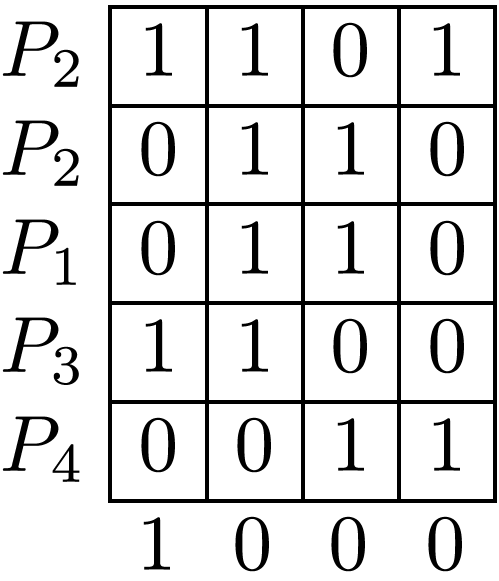
\includegraphics[width=0.5\textwidth]{image/lsss/gf2.png}
        \caption{MSP in GF2}
        \label{fig:mspgf2}    
    \end{subfigure}\hfill
    \begin{subfigure}[b]{0.48\textwidth}        
        \centering
        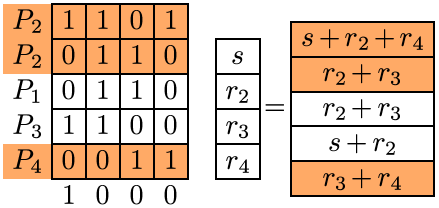
\includegraphics[width=\textwidth]{image/lsss/gf2ss.png}
        \caption{Secret Reconstruction with MSP}
        \label{fig:mspss}
    \end{subfigure}
\end{figure}
Dall'esempio, si può vedere il senso della seguente definizione:
\begin{definition}[MSP Accept]\label{def:mspacc}
Un MSP accetta un set di parti $B$ se le righe etichettate da $B$ eseguono uno span del vettore target.
\end{definition}
\section{Access Structure}
Vediamo come costruire un sistema di accesso basato su una certa policy che cambia a seconda delle parti coinvolte nel calcolo del segreto.
\begin{definition}[Access Structure]
Sia $\mathcal{P}$ un insieme di entità. Una \textbf{Struttura di Accesso} è un insieme costituito da tutti quei sottoinsiemi $X\subseteq\mathcal{P}$ che permettono di \textbf{accedere} ad un \textbf{segreto}, partendo dalla prossima definizione.\\
Diremo che una struttura d'accesso è \textbf{monotona} se la struttura \textbf{non supporta} l'operatore di negazione.
\end{definition}
\begin{example}\label{exam:policy}Consideriamo un insieme di partecipanti $P=\{P_1,P_2,P_3,P_4\}$. Supponiamo che il segreto celato dai partecipanti possa essere ricostruito \textbf{se solo se} si incontrano $P_1$ e $P_2$ o $P_1,P_3,P_4$. La struttura d'accesso \textbf{monotona} che ne deriva è l'insieme
\[A=\{[P_1,P_2],[P_1,P_3,P_4]\}\]
Il quale equivalente booleano è: $(P_1\land P_2)\lor (P_1\land P_2\land P_3)=P_1\land(P_2\lor (P_3\land P_4))$
\end{example}
\begin{remark}
Gli schemi che costruiremo \textbf{potrebbero non essere ideali}, poiché una parte potrebbe ricevere più di uno share.
\end{remark}
Questo fatto è osservabile costruendo effettivamente la matrice di accesso di controllo corrispondente alla politica da implementare.
Consideriamo la struttura d'accesso dell'esempio \ref{exam:policy}: $P_1\land(P_2\lor (P_3\land P_4))$ e deriviamo la matrice corrispondente creando un \textbf{access control tree}.
\begin{definition}[Access Control Tree]\label{def:act}
Un \textbf{Access Control Tree} è un albero binario che implementa la politica di una struttura di accesso. I nodi sono gli operatori booleani della politica, le foglie le parti che la compongono. 
\end{definition}
\begin{definition}[Access Control Matrix]\label{def:acm}
Una \textbf{Access Control Matrix} è una matrice \textbf{derivata} da un \textbf{ACT}, per implementare una Access Structure. In particolare:
\begin{itemize}
    \item Un nodo \textbf{OR} (\cref{fig:oracm}) costruisce un vettore le cui \textbf{componenti} sono \textbf{pari al segreto in ingresso} al nodo.
    \item Un nodo \textbf{AND} (\cref{fig:and2acm}, \cref{fig:and3acm}) \textbf{aumenta} la dimensione dello al numero di attori in gioco. La prima riga sarà del tipo $(X,1,\dots,1)$, le altre saranno \textbf{nulle} in ogni componente \textbf{tranne} che nella colonna \textit{i-esima}, il cui valore dovrà annullare l'1 contenuto nella prima riga.
\end{itemize}
\end{definition}
\begin{figure}[ht]
\vspace{-10pt}
     \centering
     \begin{subfigure}[b]{0.3\textwidth}
         \centering
         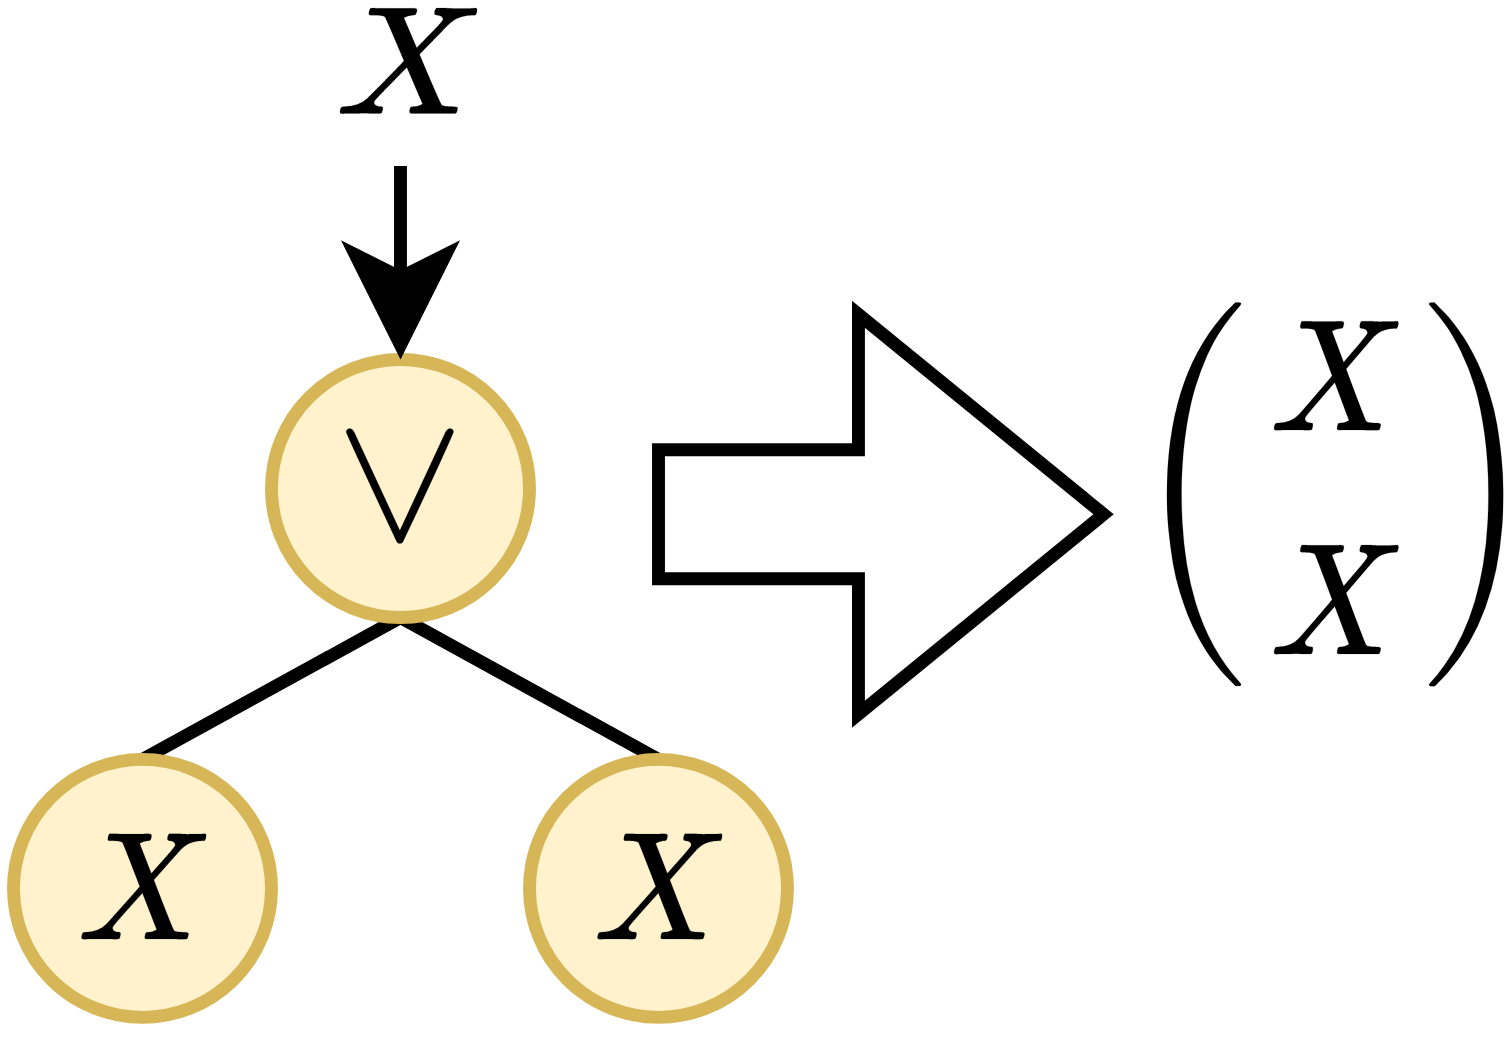
\includegraphics[width=0.9\textwidth]{image/lsss/oract.png}
         \caption{OR-ACM from OR-ACT}
         \label{fig:oracm}
     \end{subfigure}
     \hfill
     \begin{subfigure}[b]{0.3\textwidth}
         \centering
         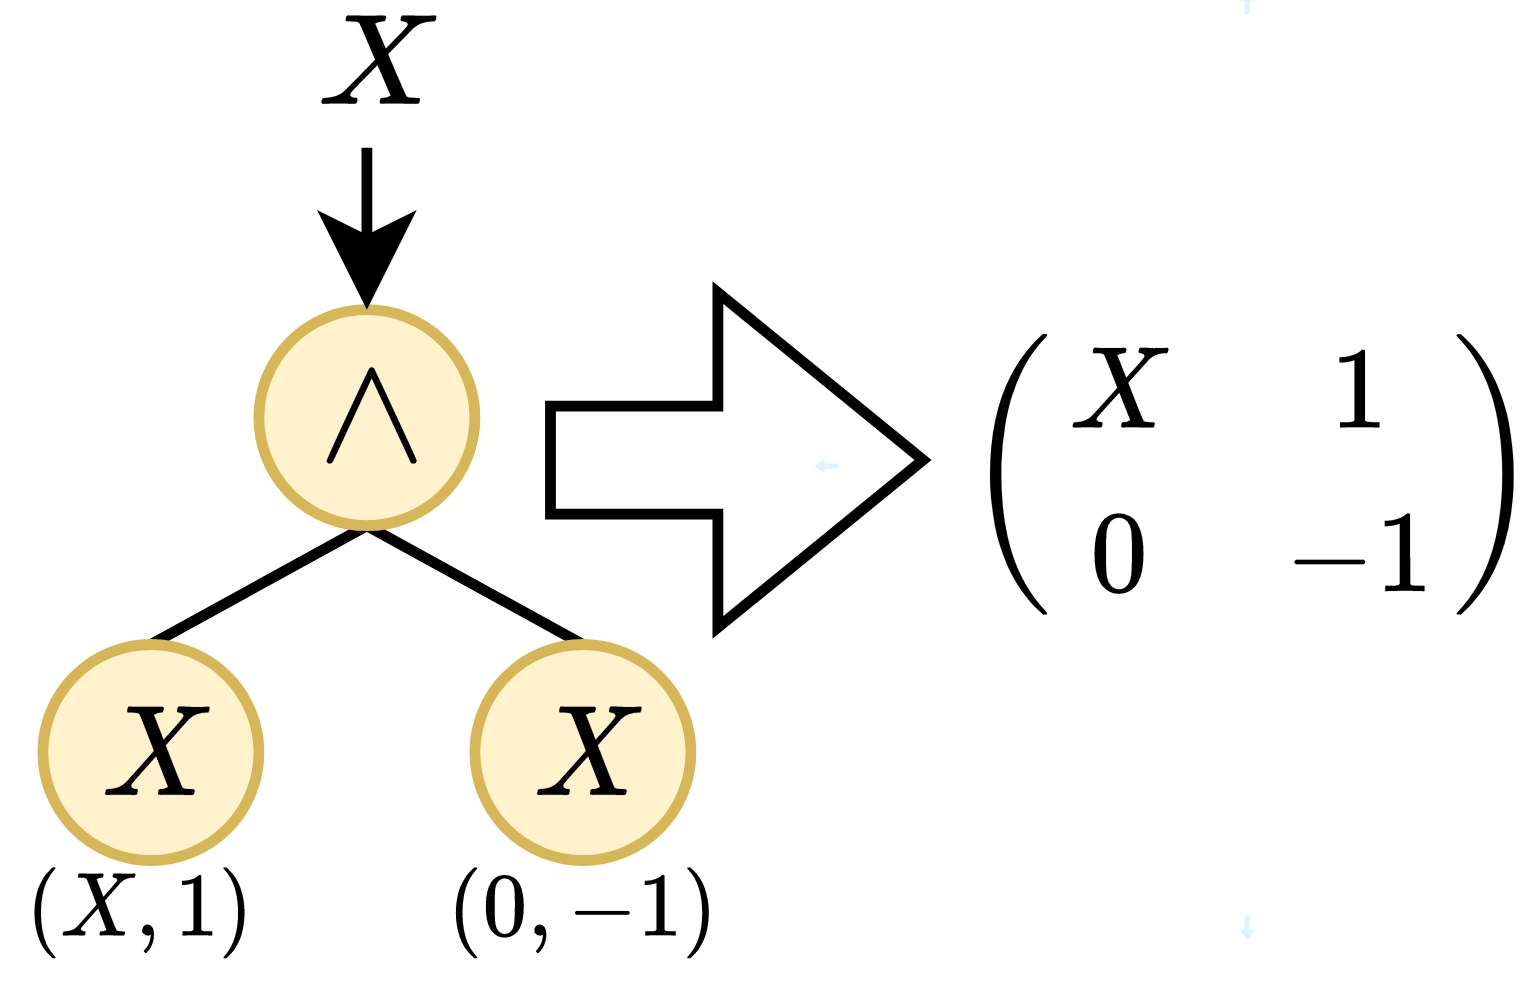
\includegraphics[width=\textwidth]{image/lsss/and2act.png}
         \caption{AND-ACM from AND-ACT}
         \label{fig:and2acm}
     \end{subfigure}
     \hfill
        \begin{subfigure}[b]{0.3\textwidth}
         \centering
         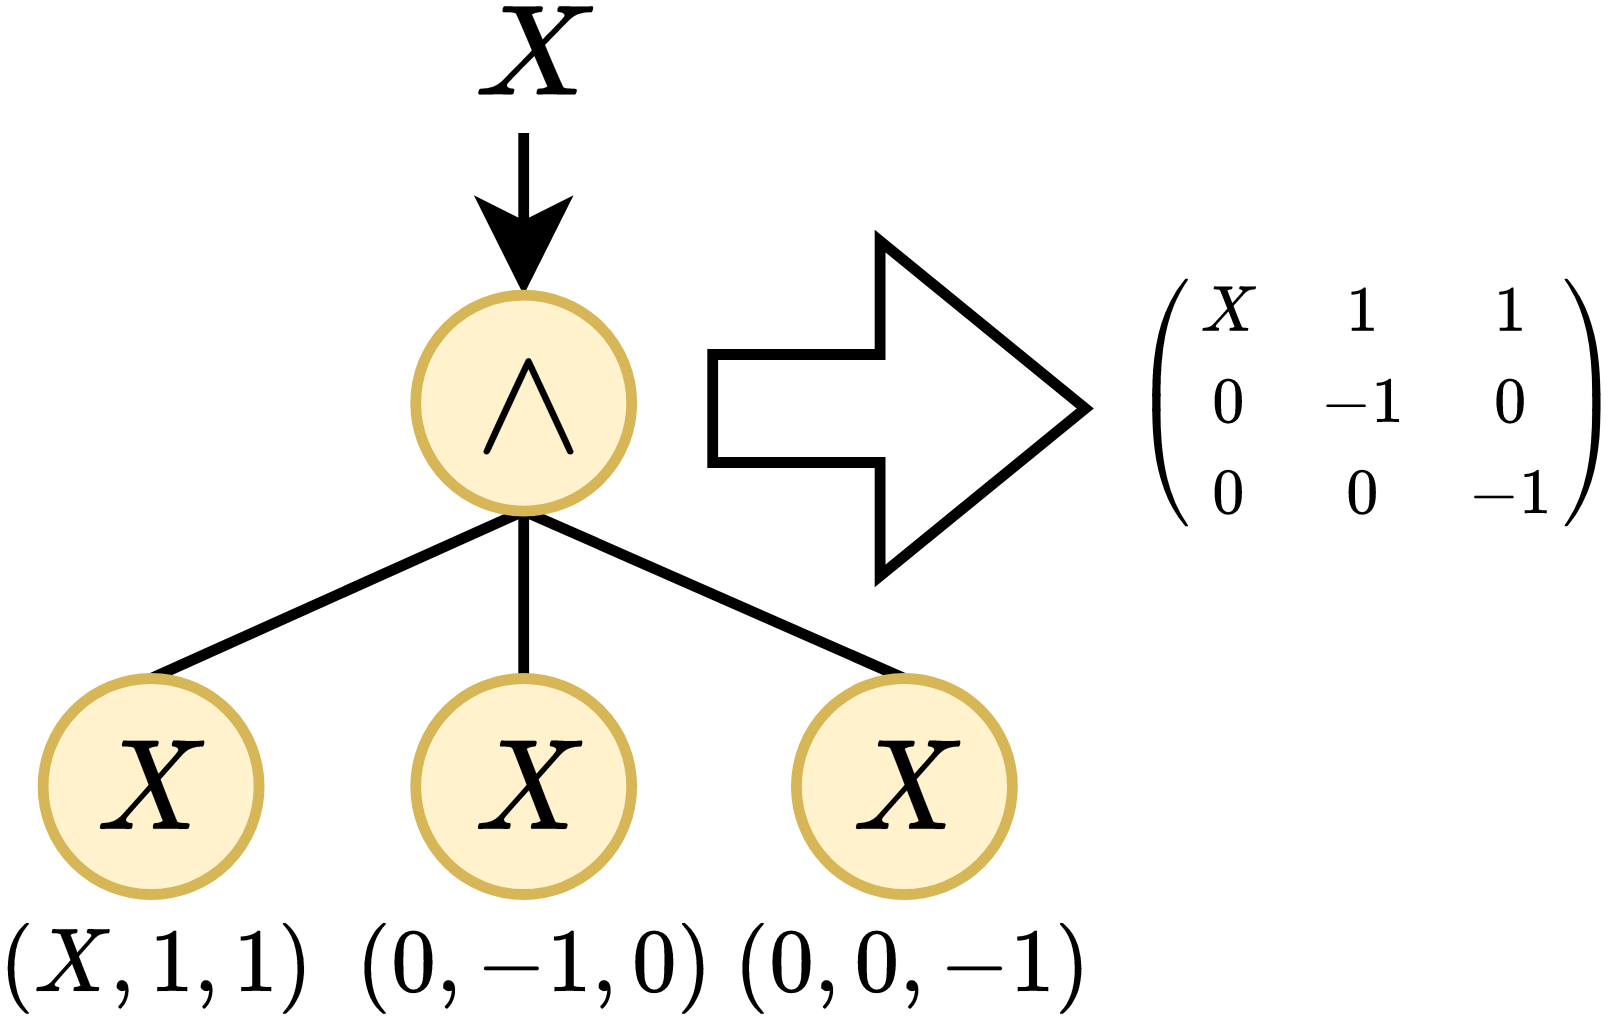
\includegraphics[width=\textwidth]{image/lsss/and3act.png}
         \caption{AND-ACM from AND-ACT }
         \label{fig:and3acm}
     \end{subfigure}
        \caption{From ACT to ACM}
        \label{fig:actacm}
\end{figure}
\begin{example}[ Access Control Matrix]
Scriviamo la ACM equivalente alla seguente proposizione: \[(P_1\land P_2)\lor (P_1\land P_2\land P_3)=P_1\land(P_2\lor (P_3\land P_4))\]
\begin{remark}
Se avessimo calcolato la ACM senza semplificarla, avremmo avuto più entry per P1 e P2 e questo non sarebbe stato uno schema \textbf{Ideale}. Tuttavia, la soluzione sub-ottimale è semplice e garantisce comunque sicurezza, senza necessariamente usare numeri primi, perché la sicurezza è garantita dalla policy.
\end{remark}
\end{example}
\begin{figure}[h]
    \centering
    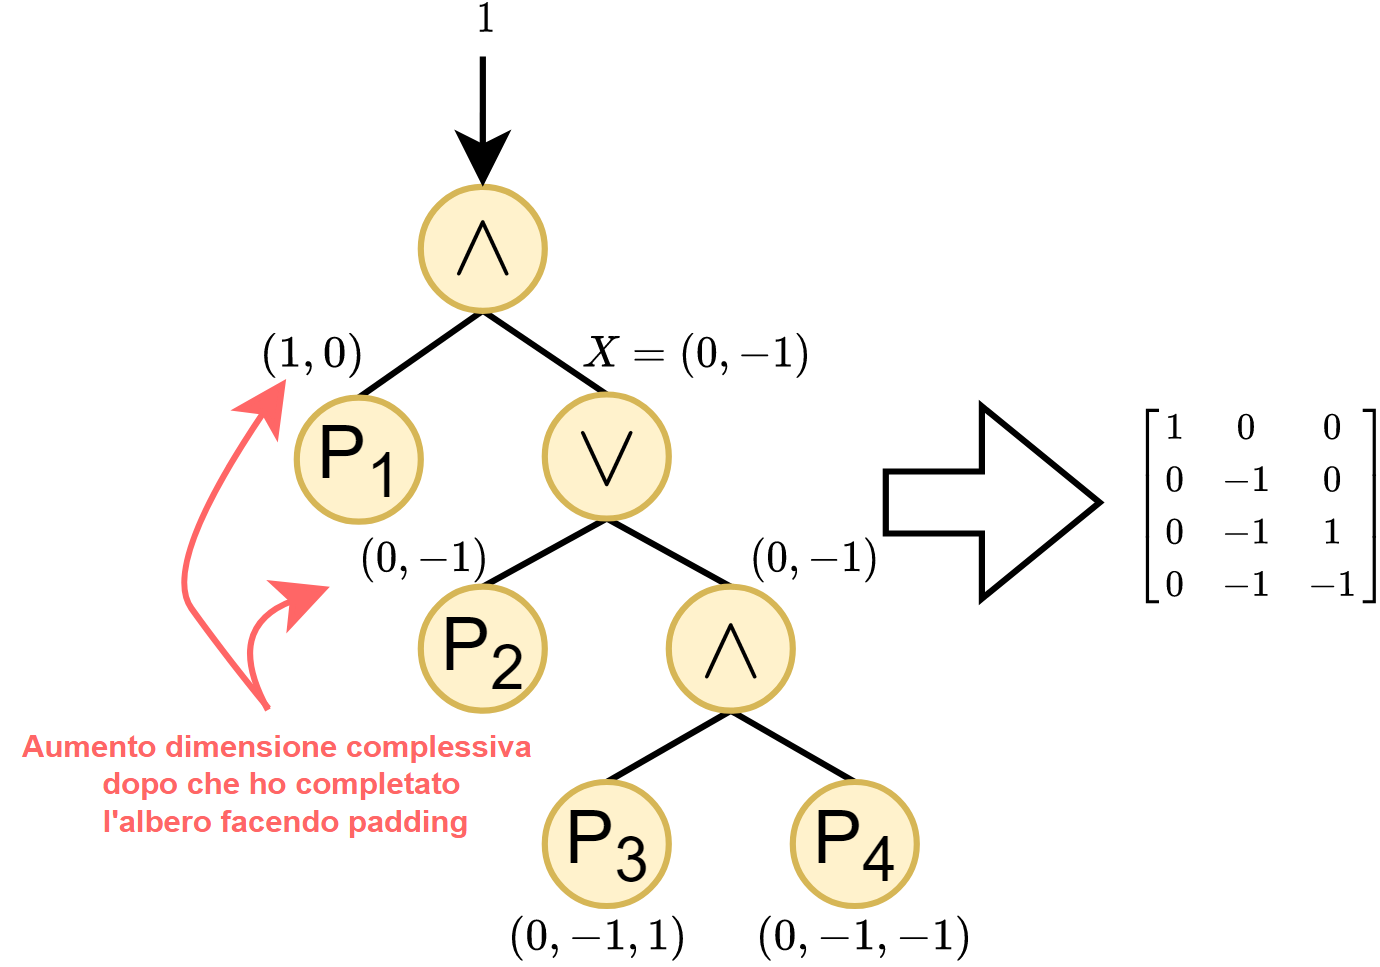
\includegraphics[width=0.5\textwidth]{image/lsss/acmex.png}
    \caption{ACM from policy}
    \label{fig:acmpol}
\end{figure}
\begin{corollary}
Con una ACM non è possibile implementare schemi ideali. E' possibile modificare lo schema per aggiungere dei \textbf{"threshold Gates"}\end{corollary}
\begin{example}
Proviamo ad implementare la policy $(A\land B)\lor(A\land C)\lor(B\land C)$  di uno schema (2,3).
\end{example}